\documentclass[11pt]{article}
\usepackage[margin=1in]{geometry}
\usepackage{amsmath,amssymb,amsthm,mathtools}
\usepackage{graphicx}
\usepackage[hidelinks]{hyperref}
\usepackage{microtype}

\newtheorem{theorem}{Theorem}
\newtheorem{lemma}{Lemma}
\newtheorem{corollary}{Corollary}
\newcommand{\Sone}{\mathbb S^1}
\newcommand{\dd}{\,\mathrm d}

\title{All-degree instability of power maps for small fractional order}
\author{Automated mathematics run \texttt{fa\_banach\_001}}
\date{11 August 2026}

\begin{document}
\maketitle

\begin{center}
\fbox{\parbox{0.91\textwidth}{\textbf{Status.}
Candidate partial result, likely valid.  The theorem below is complete, but it
does not settle existence of an arbitrary degree-one minimizer.}}
\end{center}

\begin{abstract}
For the conformally invariant $W^{s,1/s}$ energy of circle maps, a recent
preprint proves that the identity is unstable when $s<1/8$ and remarks that
the same seems true for every power map, while explicitly describing the
supporting computation as AI-generated and unverified.  We prove that
all-degree statement.  On the mode $\cos(3|d|\theta)$, the second variation at
$z\mapsto z^d$ is exactly $|d|$ times the degree-one second variation.  The
reduction follows from a cosecant root-sum identity, and a beta-integral
calculation gives the sign factor $8-1/s$.
\end{abstract}

\section{Source question and immediate context}

Mazowiecka and Schikorra ask about existence of minimizing
$W^{s,n/s}(\mathbb S^n,\mathbb S^n)$ maps of degree one
\cite[p.~6]{MS2023}.  The source passage is reproduced below.

\begin{center}

\includegraphics[width=\textwidth]{figures/open_problem_crop.png}
\end{center}

In dimension one, Martino--Mazowiecka--Schikorra prove that the identity is
not minimizing when $s<1/8$ \cite[Theorem~1.1]{MMS2026}.  Their footnote says
that every $z^d$ appears to lose positive definiteness in the same regime, but
labels the trigonometric computation ``AI generated, unverified.''

\begin{center}
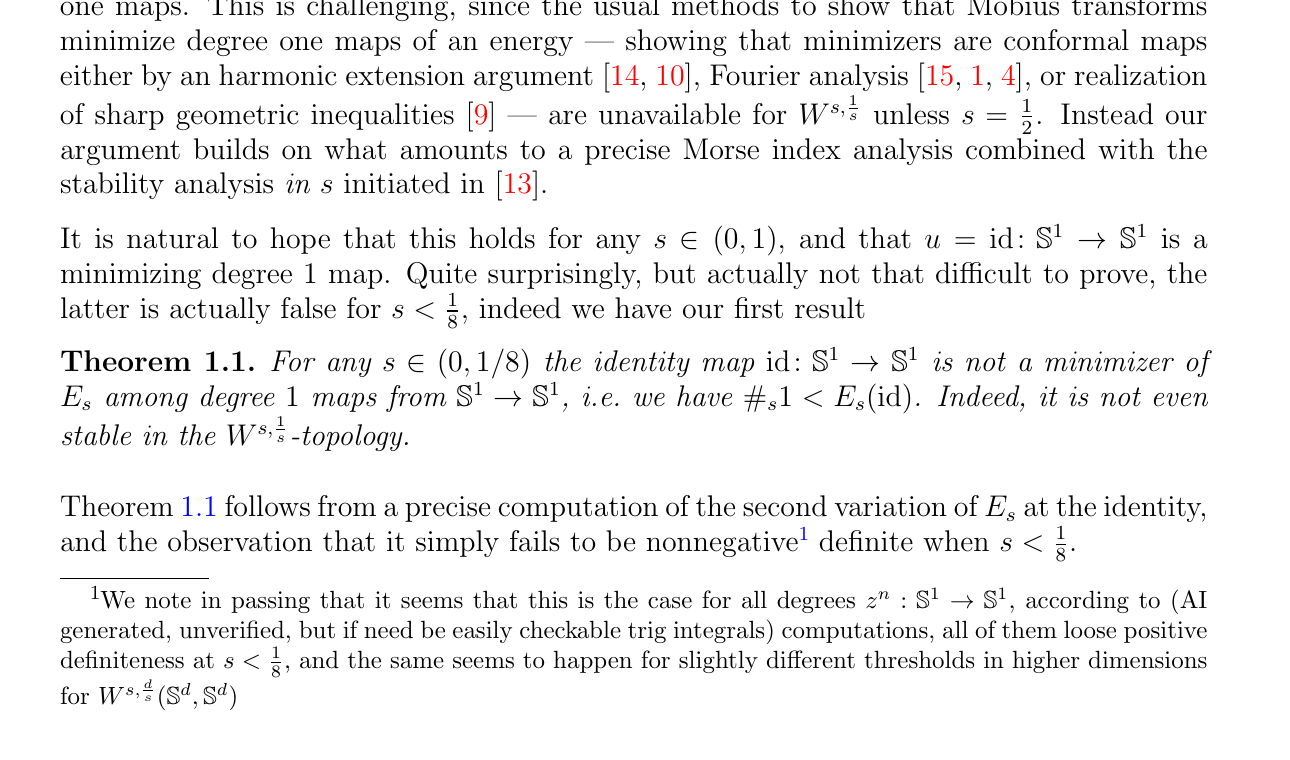
\includegraphics[width=\textwidth]{figures/unverified_all_degree_claim_crop.png}
\end{center}

The theorem below supplies a proof of that all-degree statement.  It is
substantial progress around the source question, but does not prove or
disprove existence of a different degree-one minimizer.

\section{Definitions and statement}

For $s\in(0,1)$ put $p=1/s$ and define, for $u:\Sone\to\Sone$,
\begin{equation}\label{eq:energy}
 E_s(u)=\int_0^{2\pi}\!\int_0^{2\pi}
 \frac{|u(e^{i\theta})-u(e^{i\sigma})|^p}
 {|e^{i\theta}-e^{i\sigma}|^2}\,\dd\theta\,\dd\sigma.
\end{equation}
For $d\in\mathbb Z\setminus\{0\}$ let $u_d(e^{i\theta})=e^{id\theta}$ and
write $q=|d|$.  Consider the smooth, degree-$d$ path
\begin{equation}\label{eq:path}
 u_{d,\varepsilon}(e^{i\theta})
 =\exp\!\left(i\bigl(d\theta+\varepsilon\cos(3q\theta)\bigr)\right).
\end{equation}

\begin{theorem}[Exact all-degree negative mode]\label{thm:main}
Let $s\in(0,1/8)$, $p=1/s$, and $d\ne0$.  For the path
\eqref{eq:path},
\begin{equation}\label{eq:exact-second}
 \left.\frac1p\frac{\dd^2}{\dd\varepsilon^2}
 E_s(u_{d,\varepsilon})\right|_{\varepsilon=0}
 =q(8-p)2^{p+1}\pi^{3/2}
 \frac{\Gamma((p+1)/2)}{\Gamma(3+p/2)}<0.
\end{equation}
Consequently $u_d$ is not a local minimizer of $E_s$ within its degree class,
even against smooth perturbations.  In particular,
\[
 \inf_{\deg u=d}E_s(u)<E_s(u_d)=qE_s(u_1).
\]
\end{theorem}

\section{Proof intuition}

The energy is translation invariant in the angular variables, so its second
variation at a power map is a Fourier multiplier.  The target angle winds
$q$ times while the domain angle winds once; this changes the target factors
to $\sin(qt/2)$ but leaves a domain denominator $\sin^2(t/2)$.  Choosing the
frequency $3q$ synchronizes the perturbation with every target winding.
Partitioning the $t$-circle into $q$ arcs then turns all target factors into
their degree-one versions.  The only apparent obstruction is the sum of the
$q$ domain denominators, and the cosecant root-sum identity collapses it
exactly, leaving a factor $q$.  The remaining degree-one beta integral has
sign $8-p$.

\section{Proof}

We first compute the quadratic form at an arbitrary power map.  For a smooth
real $2\pi$-periodic function $\eta$, set
\[
 v_\varepsilon(\theta)=e^{i(d\theta+\varepsilon\eta(\theta))}.
\]
Write $a=e^{id\theta}$, $b=e^{id\sigma}$,
$t=\theta-\sigma$, and $\Delta=dt$.  At $\varepsilon=0$, if
$D=a-b$, $V=\partial_\varepsilon(v_\varepsilon(\theta)-
v_\varepsilon(\sigma))$, and $W=\partial_\varepsilon^2(cdots)$, then
\[
 V=\eta(\theta)a^\perp-\eta(\sigma)b^\perp,
 \qquad
 W=-\eta(\theta)^2a+\eta(\sigma)^2b.
\]
Elementary scalar-product identities give
\begin{align*}
 \langle D,V\rangle
 &=\sin\Delta\,[\eta(\theta)-\eta(\sigma)],\\
 |V|^2+\langle D,W\rangle
 &=\cos\Delta\,[\eta(\theta)-\eta(\sigma)]^2.
\end{align*}
The first variation vanishes: after writing $\theta=\sigma+t$, its inner
integral contains
$\int_0^{2\pi}(\eta(\sigma+t)-\eta(\sigma))\dd\sigma=0$.

Using
\[
 \frac1p\frac{\dd^2}{\dd\varepsilon^2}|D_\varepsilon|^p
 =(p-2)|D|^{p-4}\langle D,V\rangle^2
 +|D|^{p-2}(|V|^2+\langle D,W\rangle),
\]
and $|D|=2|\sin(\Delta/2)|$, we obtain
\begin{equation}\label{eq:Qkernel}
 \mathcal Q_{p,d}(\eta)
 :=\left.\frac1p\frac{\dd^2}{\dd\varepsilon^2}
 E_s(v_\varepsilon)\right|_{0}
 =\int_0^{2\pi}\!\int_0^{2\pi}
 K_{p,d}(\theta-\sigma)
 [\eta(\theta)-\eta(\sigma)]^2\dd\theta\dd\sigma,
\end{equation}
where
\begin{equation}\label{eq:kernel}
 K_{p,d}(t)=
 \frac{|2\sin(dt/2)|^{p-2}}
 {4\sin^2(t/2)}\left(p\cos^2(dt/2)-1\right).
\end{equation}
For $p>8$ all differentiations and integrals are justified directly by
dominated convergence; the apparent singularities in \eqref{eq:kernel} are
removable after multiplication by the phase difference.

We now record the exact folding identity.

\begin{lemma}[Cosecant root sum]\label{lem:rootsum}
For every integer $q\ge1$ and $x\notin2\pi\mathbb Z$,
\begin{equation}\label{eq:rootsum}
 \sum_{j=0}^{q-1}
 \csc^2\!\left(\frac{x+2\pi j}{2q}\right)
 =q^2\csc^2(x/2).
\end{equation}
\end{lemma}

\begin{proof}
The factorization of $\sin(qz)$, or logarithmic differentiation of it, gives
\[
 \sum_{j=0}^{q-1}\cot\!\left(z+\frac{\pi j}{q}\right)
 =q\cot(qz).
\]
Differentiate and put $z=x/(2q)$.
\end{proof}

Take $\eta(\theta)=\cos(3q\theta)$.  Integrating first in $\sigma$ in
\eqref{eq:Qkernel} yields
\begin{equation}\label{eq:mode}
 \mathcal Q_{p,d}(\eta)
 =2\pi\int_0^{2\pi}K_{p,d}(t)
 (1-\cos(3qt))\dd t.
\end{equation}
The kernel is unchanged when $d$ is replaced by $q=|d|$.  Partition the
integral into $q$ consecutive intervals and on the $j$th interval put
$t=(x+2\pi j)/q$.  All numerator terms become their degree-one versions.
Using Lemma~\ref{lem:rootsum},
\begin{align}
 \int_0^{2\pi}K_{p,d}(t)(1-\cos(3qt))\dd t
 &=q\int_0^{2\pi}K_{p,1}(x)(1-\cos(3x))\dd x.
 \label{eq:fold}
\end{align}
Therefore
\begin{equation}\label{eq:q-times}
 \mathcal Q_{p,d}(\cos(3q\cdot))
 =q\,\mathcal Q_{p,1}(\cos(3\cdot)).
\end{equation}

It remains to evaluate the degree-one form.  Setting $x=2r$ in
\eqref{eq:mode} and using
$\sin(3r)=\sin r(4\cos^2r-1)$ gives
\begin{equation}\label{eq:beta-start}
 \mathcal Q_{p,1}(\cos(3\cdot))
 =2^{p-1}\pi\int_0^\pi
 \sin^{p-2}r\,(p\cos^2r-1)(4\cos^2r-1)^2\dd r.
\end{equation}
Let
\[
 A_k=\int_0^\pi\sin^{p-2}r\cos^{2k}r\dd r
 =B\!\left(\frac{p-1}{2},k+\frac12\right).
\]
Relative to $A_0$,
\[
 \frac{A_1}{A_0}=\frac1p,\qquad
 \frac{A_2}{A_0}=\frac{3}{p(p+2)},\qquad
 \frac{A_3}{A_0}=\frac{15}{p(p+2)(p+4)}.
\]
Expanding the polynomial in \eqref{eq:beta-start}, the bracketed integral is
\begin{align*}
 16pA_3-(8p+16)A_2+(p+8)A_1-A_0
 &=A_0\frac{16(p-1)(8-p)}{p(p+2)(p+4)}.
\end{align*}
Since
$A_0=\sqrt\pi\,\Gamma((p-1)/2)/\Gamma(p/2)$, the gamma recurrence yields
\begin{equation}\label{eq:q1}
 \mathcal Q_{p,1}(\cos(3\cdot))
 =(8-p)2^{p+1}\pi^{3/2}
 \frac{\Gamma((p+1)/2)}{\Gamma(3+p/2)}.
\end{equation}
Combining \eqref{eq:q-times} and \eqref{eq:q1} proves
\eqref{eq:exact-second}.  It is strictly negative for $p>8$.

Finally, the path \eqref{eq:path} has degree $d$ for every $\varepsilon$ and
converges smoothly, hence in $W^{s,p}$, to $u_d$.  Taylor expansion and the
vanishing first variation imply
$E_s(u_{d,\varepsilon})<E_s(u_d)$ for all sufficiently small nonzero
$\varepsilon$.  The identity $E_s(u_d)=qE_s(u_1)$ follows from the same
partition and Lemma~\ref{lem:rootsum}, now applied directly to
\eqref{eq:energy}.  This completes the proof of Theorem~\ref{thm:main}.

\section{Verification and limitations}

The included script \texttt{code/verify\_multiplier.py} evaluates
\eqref{eq:mode} with 50-digit quadrature for
$p\in\{9,10,12\}$ and $q\in\{1,2,3,5\}$.  It reproduces
$q$ times \eqref{eq:q1} to roughly $10^{-47}$ or better.  This is only a
regression check; the proof is the exact argument above.

This theorem does not settle the source existence question.  In particular,
when $s<1/8$ a non-power degree-one map might still attain the infimum.  The
endpoint $s=1/8$ is degenerate for the selected mode, and neither other maps
nor higher-dimensional analogues are addressed.

A bounded novelty check on 11 August 2026 searched the run indexes and the
official arXiv API using the exact titles and combinations of ``power maps,''
``fractional harmonic,'' ``second variation,'' ``degree one,'' ``$W^s$,'' and
``positive definiteness.''  The exact degree-one query returned only
arXiv:2606.15644v1, whose footnote explicitly says the all-degree computation
is unverified; the closest all-degree and second-variation queries returned no
records.  No rigorous prior proof was found.  The novelty assessment is
plausible, not an exhaustive certification.

\paragraph{Human-review recommendation.}
Check equations \eqref{eq:kernel}, \eqref{eq:fold}, and the beta-integral
normalization.  These are the only nontrivial algebraic transitions.

\begin{thebibliography}{9}

\bibitem{MS2023}
K.~Mazowiecka and A.~Schikorra,
\emph{Minimal $W^{s,n/s}$-harmonic maps in homotopy classes},
J. Lond. Math. Soc. 108 (2023), 742--836;
arXiv:2006.07138.

\bibitem{MMS2026}
D.~Martino, K.~Mazowiecka, and A.~Schikorra,
\emph{Minimizing and non-minimizing degree one
$W^{s,1/s}$-harmonic maps between spheres},
arXiv:2606.15644v1 (2026).

\end{thebibliography}

\end{document}

